\documentclass[tikz,border=4pt]{standalone}
% Estilo común de los diagramas de bloques (se usa con \input en cada standalone)
\usepackage[defaultsans,scale=0.92]{lato}
\usepackage{libertinust1math}
\usepackage{xcolor,amsmath}
\usepackage{tikz}
\usetikzlibrary{positioning,arrows.meta,calc,shapes.geometric}
\usepackage{../../notacion}
\definecolor{ctrlazul}{HTML}{1E5AA8}\definecolor{ctrlnoche}{HTML}{14213D}
\definecolor{ctrlcoral}{HTML}{D1495B}\definecolor{ctrlverde}{HTML}{2A9D8F}
\definecolor{ctrlambar}{HTML}{E09F3E}\definecolor{ctrlgris}{HTML}{5C677D}
\definecolor{ctrlvioleta}{HTML}{6C4AB6}\definecolor{ctrlteal}{HTML}{0F7173}
\tikzset{
  >={Stealth[length=2.4mm]}, every node/.style={font=\small},
  bloque/.style={draw=ctrlnoche,fill=ctrlazul!7,thick,rounded corners=1.5pt,minimum height=9mm,minimum width=13mm,inner sep=4pt},
  suma/.style={draw=ctrlnoche,thick,circle,inner sep=0pt,minimum size=6mm},
  senal/.style={->,thick,draw=ctrlnoche},
  rot/.style={font=\footnotesize,text=ctrlgris},
}

\begin{document}
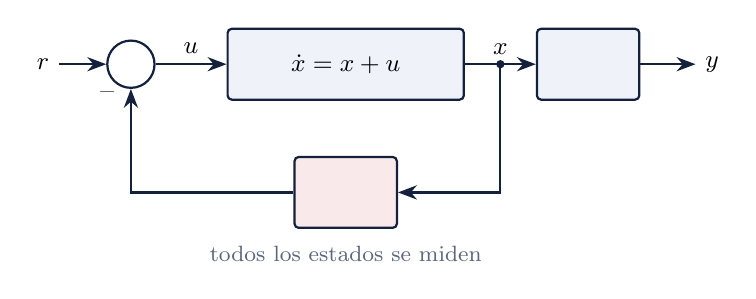
\begin{tikzpicture}[node distance=9mm]
  \node (r) {$r$}; \node[suma,right=6mm of r] (S) {};
  \node[bloque,right=9mm of S,minimum width=30mm,align=center] (P) {$\dot x=\Am x+\Bm u$};
  \node[bloque,right=9mm of P] (C) {$\Cm$};
  \node[right=7mm of C] (y) {$y$};
  \coordinate (n) at ($(P.east)!0.5!(C.west)$);
  \node[bloque,below=7mm of P,fill=ctrlcoral!12] (K) {$\Km$};
  \draw[senal] (r)--(S); \draw[senal] (S)--node[above]{$u$}(P); \draw[senal] (P)--(C); \draw[senal] (C)--(y);
  \fill[ctrlnoche] (n) circle (1.5pt); \node[above] at (n) {$x$};
  \draw[senal] (n)|-(K); \draw[senal] (K)-|(S); \node[rot] at ($(S)+(-3mm,-3.5mm)$) {$-$};
  \node[rot,below=1mm of K] {todos los estados se miden};
\end{tikzpicture}
\end{document}
